%
% File nodalida2017.tex
%
% Contact beata.megyesi@lingfil.uu.se
%
% Based on the instruction file for Nodalida 2015 and EACL 2014
% which in turn was based on the instruction files for previous 
% ACL and EACL conferences.

\documentclass[11pt]{article}
\usepackage{nodalida2017}
\usepackage{mathptmx}
%\usepackage{txfonts}
\usepackage{url}
\usepackage{latexsym}
\usepackage{tikz-dependency}
\usepackage[plain]{fancyref}
\special{papersize=210mm,297mm} % to avoid having to use "-t a4" with dvips 
%\setlength\titlebox{6.5cm}  % You can expand the title box if you really have to

\title{Universal Dependencies for Swedish Sign Language}

\author{Robert {\"O}stling, Carl B{\"o}rstell,
    Moa G{\"a}rdenfors, Mats Wir{\'e}n \\
  Department of Linguistics \\
  Stockholm University \\
  {\tt \{robert,calle,moa.gardenfors,mats.wiren\}@ling.su.se} \\}

\date{}

\begin{document}
\maketitle
\begin{abstract}
    We describe the first effort to annotate a signed language with syntactic
    dependency structure: the Swedish Sign Language portion of the
    Universal Dependencies treebanks.
    The visual modality presents some unique challenges in analysis and
    annotation, such as the possibility of
    both hands articulating separate signs simultaneously, which has
    implications for the concept of \emph{projectivity} in dependency grammars.
    Our data is sourced from the Swedish Sign Language Corpus,
    and if used in conjunction these resources contain very richly
    annotated data: dependency structure and parts of speech,
    video recordings, signer metadata, and since the whole material is
    also translated into Swedish the corpus is also a parallel text.
\end{abstract}

\section{Introduction}

The Universal Dependencies (UD) project \cite{Nivre2016ud} 
has produced a language-independent but extensible standard for
morphological and syntactic annotation using a formalism based on
dependency grammar. This standard has been used to create the Universal
Dependencies treebanks \cite{ud14}, which in its latest release at the time of
writing (version 1.4) contains 64 treebanks in 47 languages---one of which is
Swedish Sign Language (SSL, ISO 639-3: \textsc{swl}), the topic of this
article.

There are very few sign languages for which there are corpora. Most of the
available sign language corpora feature only simple sign segmentation and
annotations, often also with some type of translation into a spoken language
(either as written translations or as spoken voice-overs). Sign language
corpora with more extensive syntactic annotation is limited to Australian Sign
Language, which contains some basic syntactic segmentation and annotation
\cite{Johnston2014annotation}. Apart from this, smaller parts of the corpora
of Finnish Sign Language \cite{Jantunen2016corpus} and Polish Sign Language
\cite{Rutkowski2016corpus}, have had some syntactic segmentation and analysis,
and another such project is under way on British Sign
Language.\footnote{\url{http://www.bslcorpusproject.org/projects/bsl-syntax-project/}}

To the best of our knowledge, we present the first dependency annotation and
parsing experiments with sign language data. This brings us one step closer to
the goal of bridging the gap in availability between written, spoken and sign
language natural language processing tools.

\section{Universal Dependencies}

The Universal Dependencies project aims to provide uniform morphological and
syntactic (in the form of dependency trees) annotations across languages
\cite{Nivre2016ud}.\footnote{Note that our work predates version 2 of the UD
guidelines, and is based on the first version.}
Built on a language-universal common core of 17 parts of speech and
40 dependency relations, there are also language-specific guidelines which
interpret and when necessary extend those in the context of a given language.

\section{Swedish Sign Language}

Swedish Sign Language (SSL) is the main sign language of the Swedish Deaf
community.\footnote{Capital D ``Deaf'' is generally used to refer to the
language community as a cultural and linguistic group, rather than `deaf' as a
medical label.} It is estimated to be used by at least 10,000 as one of their
primary languages, and is the only sign language to be recognized in Swedish
law, giving it a special status alongside the official minority languages
\cite{Ahlgren2006sou,Parkvall2015siffror}. The history of SSL goes back at
least 200 years, to the inauguration of the first Deaf school in Sweden, and
has also influenced the two sign languages of Finland (i.e.~Finnish Sign
Language and Finland-Swedish Sign Language) with which SSL can be said to be
related \cite{Bergman2010transmission}.

\section{Data source}

The SSL Corpus Project ran during the years 2009--2011 with the intention to
establish the first systematically designed and publicly available corpus of
SSL, resulting in the SSL Corpus (SSLC). Approximately 24 hours of video data
of pairs of signers conversing was recorded, comprising 42 signers of
different age, gender, and geographical background, spanning 300 individual
video files \cite{Mesch2012signed}. The translation and annotation work is
still on-going, with new releases being made available online as the work
moves forward. The last official release of the SSLC includes just under 7
hours of video data \cite{Mesch2012dataset} along with annotation files
containing 53,625 sign tokens across 6,197 sign types
\cite{Mesch2016annotated}. 

The corpus is annotated using the ELAN software \cite{Wittenburg2006elan}, and
the annotation files are distributed in the corresponding XML-based
\texttt{.eaf} format. Each annotation file contains tiers on which annotations
are aligned with the video file, both video and annotation tiers being visible
in the ELAN interface (see \Fref{fig:sslc_elan}). The SSLC annotation files
currently include tiers for sign glosses, and others for Swedish translations.
Sign glosses are written word labels that represent signs with approximate
meanings (e.g. \textsc{pro1} for a first person pronoun). The sign gloss
annotation tiers are thus segmented for lexical items (i.e.~individual signs),
and come in pairs for each signer---each tier representing one of the signer's
hands (one tier for the so-called \textit{dominant hand}, and another for the
\textit{non-dominant hand}) \cite{Mesch2015gloss}.\footnote{The dominant hand
is defined as the hand preferred by a signer when signing a one-handed sign.}
Sign glosses also contain a part-of-speech (PoS) tag which have been derived
from manually correcting the output of a semi-automatic method for
cross-lingual PoS tagging \cite{Ostling2015enriching}. The translation tier is
segmented into longer chunks, representing stretches of discourse that can be
represented by an idiomatic Swedish translation. However, the translation
segmentations do not represent clausal boundaries in either SSL or Swedish
\cite{Borstell2014segmenting}. More recently, a portion of the SSLC was
segmented into clausal units and annotated for basic syntactic roles
\cite{Borstell2016syntactic}, which led to the current UD annotation work.
\Fref{fig:sslc_elan} shows the basic view of the SSLC videos and annotations
in the ELAN software, with tiers for sign glosses and translations on the
video timeline.

\begin{figure*}[p]
	\centering
	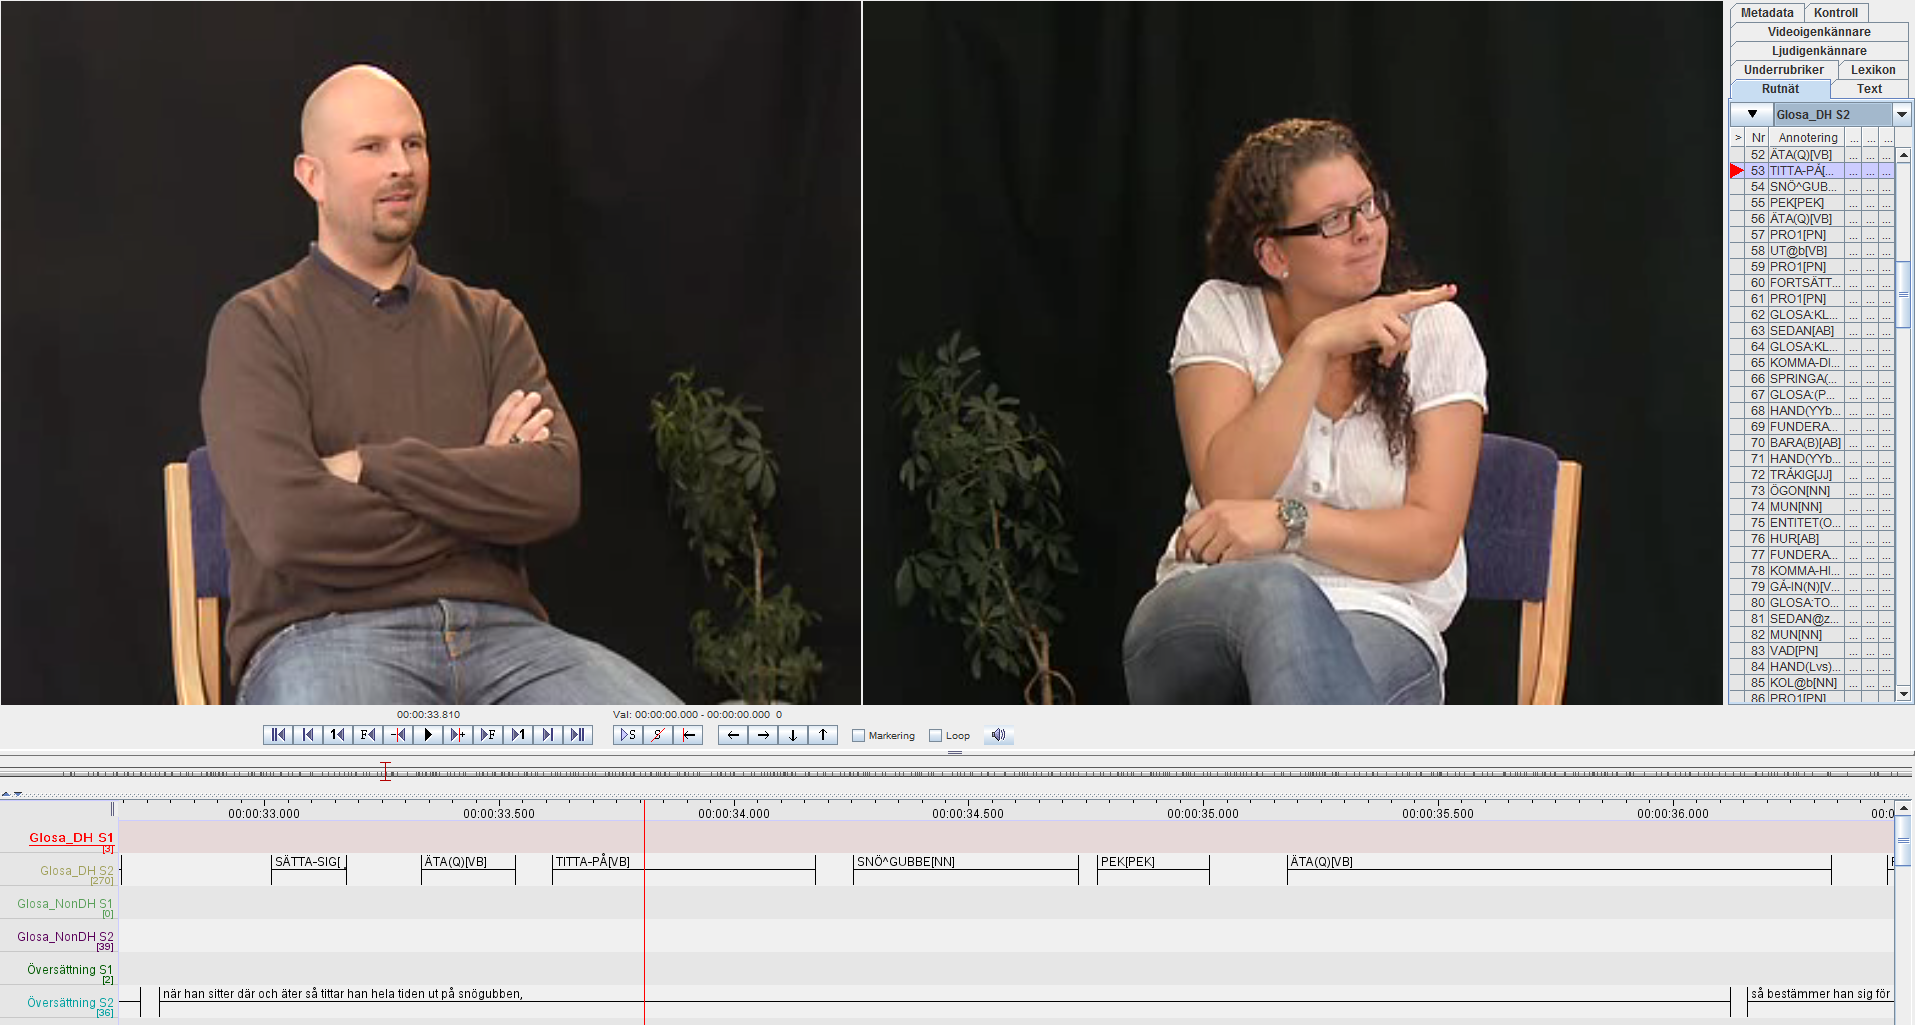
\includegraphics[width=0.9\textwidth]{sslc_elan.png}
	\caption{Screenshot of an SSLC file in ELAN. This is the material we base
    our dependency annotations on, and the annotator can easily view the
    source video recording.}
	\label{fig:sslc_elan}
\end{figure*}

\section{Annotation procedure and principles for SSL}
\label{sec:annotation}

\begin{figure*}[p]
	\centering
	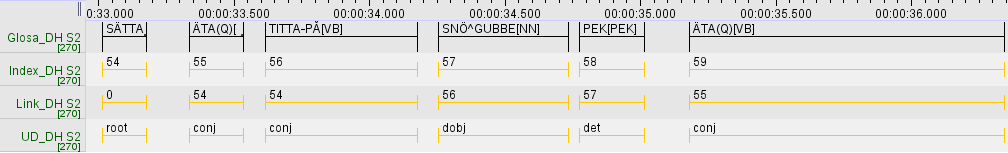
\includegraphics[width=0.9\textwidth]{sslc_elan_ud.png}
	\caption{Screenshot zooming into the UD annotation tiers and
    sign--dependency linking for the utterance from \Fref{fig:sslc_elan}.
    This is the interface used by the annotator.}
	\label{fig:sslc_elan_ud}
\end{figure*}

\begin{figure*}[p]
\centering
\begin{dependency}[theme = default, label style={scale=1.0}]
   \begin{deptext}[column sep=1em]
      \texttt{verb} \& \texttt{verb} \& \texttt{verb} \& \texttt{noun} \& \texttt{det} \& \texttt{verb} \\
      \textsc{s{\"a}tta-sig} \& \textsc{{\"a}ta}(Q) \& \textsc{titta-p{\aa}} \& \textsc{sn{\"o}{\string^}gubbe} \& \textsc{pek} \& \textsc{{\"a}ta}(Q) \\
      \textsc{sit-down} \& \textsc{eat}(Q) \& \textsc{look-at} \& \textsc{snow{\string^}old-man} \& \textsc{point} \& \textsc{eat}(Q) \\
   \end{deptext}
   \deproot{1}{root}
   \depedge{1}{2}{conj}
   \depedge{1}{3}{conj}
   \depedge{3}{4}{dobj}
   \depedge{4}{5}{det}
   \depedge[arc angle=50]{2}{6}{conj}
   \node (translation) [below left of = \wordref{1}{1}, xshift=6cm, yshift=-2em] {
   `He is sitting there eating looking out at
   the snowman.'};
\end{dependency}
\caption{The example from \Fref{fig:sslc_elan} and \Fref{fig:sslc_elan_ud}
with dependency annotations visualized.
The (Q) suffix on the \textsc{{\"a}ta}(Q) gloss indicates which of the
multiple signs for `eat' in SSL is used in this case.}
\label{fig:ssl_dep}
\end{figure*}

For practical purposes, annotation was performed by extending the ELAN
files of our source material from the SSLC project (see
\Fref{fig:sslc_elan_ud} for an example). These annotations were automatically
converted to the CoNLL-U format used by Universal Dependencies.

The annotation of UD based syntactic structure started by coming up with a
procedure for annotating a signed language using ELAN. Signed language is more
simultaneous than spoken language, particularly in the use of paired parallel
articulators in form of the signer's two hands
\cite{Vermeerbergen2007simultaneity}.  We handle this by allowing signs from
both hands into the same tree structure, which leads to well-formed trees
consistent with the dependency grammar formalism's single-head, connectedness
and acyclicity constraints.  These trees can however have some unusual
properties compared to spoken languages.  For the purpose of conforming to the
CoNLL-U data format, which requires an ordered sequence of tokens, we sort
signs by their chronological order. The chronological order spans both sign
tiers per signer, and is defined as the onset time of each sign annotation. In
the case of two signs on each hand tier (i.e.~dominant vs.~non-dominant hand)
having identical onsets, favor is given to signs articulated by the signer's
dominant hand.  This working definition is by no means the only reasonable
linearization, which means that the notion of projectivity to some extent
loses its meaning.  A tree can be considered projective or non-projective
depending on how the ordering of simultaneously articulated signs is
defined---assuming one wants to impose such an ordering in the first place.
%An alternative to adapting the sign language data to fit the formalism, as we
%have done in order to meet the requirements of the UD standards, is obviously
%to construct a formalism adapted specifically to sign languages.  This is the
%path chosen by \newcite{Dubot2014ahybrid} in their parsing experiments.
%Consider the example in \Fref{fig:ssl_dep}, which is non-projective
%due to the link between the two instances of \textsc{eat},
%but exchanging the order of \textsc{eat} and \textsc{look-at} would
%give us a projective tree.

Because the source material contains no segmentation above the sign level,
we decided to use a bottom-up annotation procedure where subtrees were
connected until we could find no more suitable mergers. In other words,
the segmentation is entirely based on syntactic structure. The resulting fully
connected trees were then used as ``sentences'' in the CoNLL-U format.

One peculiar feature of many sign languages is the repetition of verbs, sometimes referred to as \textit{verb sandwiches}, in which one verb occurs in the middle of a sentence and also repeated at the end \cite{Bergman1994ideophones}. Such a construction is found in \Fref{fig:ssl_dep}, in which the verb \textsc{eat} appears in two places. Whereas verb chains (i.e.~multiple verbs in one clause) were treated as coordinated elements linked to the \texttt{root} verb using the label \texttt{conj}, we decided to treat repeated verbs differently by labeling the repeated verb as a coordinated element linked to its first occurrence (see \Fref{fig:ssl_dep}).
%Because of this, and because the sign gloss annotation tiers are separate for the individual hands, we had to include one set of annotation tiers for each hand (i.e.~two per signer, or four per annotation file since there are two signers). We came up with an alignment system that combined the alignment with sign annotations and the linking of dependency relations between signs. Each tier set consisted of three tiers: \texttt{Index}; \texttt{Link}; and \texttt{UD}. The three tiers were generated using [[[technical stuff]]], creating dependent tiers to the sign gloss tiers. On the \texttt{Index} tier, each sign was assigned an integer based on its chronological position in the file (in case of overlapping signs, the onset was given precedence, or the dominant hand if onsets were identical)---this was done using a script iterating over all annotation files. On the \texttt{Link} tier, the index of the sign on which the sign was dependent was entered into each annotation cell. Lastly, on the \texttt{UD} tier, the dependency relation of a sign was entered into its annotation cell. Later, a custom script extracted this manually annotated data, and converted it into the CoNLL-U format used by the UD project. The method of using ELAN for linking and annotating dependency relations on parallel annotation tiers is shown in Figure~\ref{fig:sslc_elan_ud}.

\section{Treebank statistics}

\begin{figure}[tb]
	\centering
	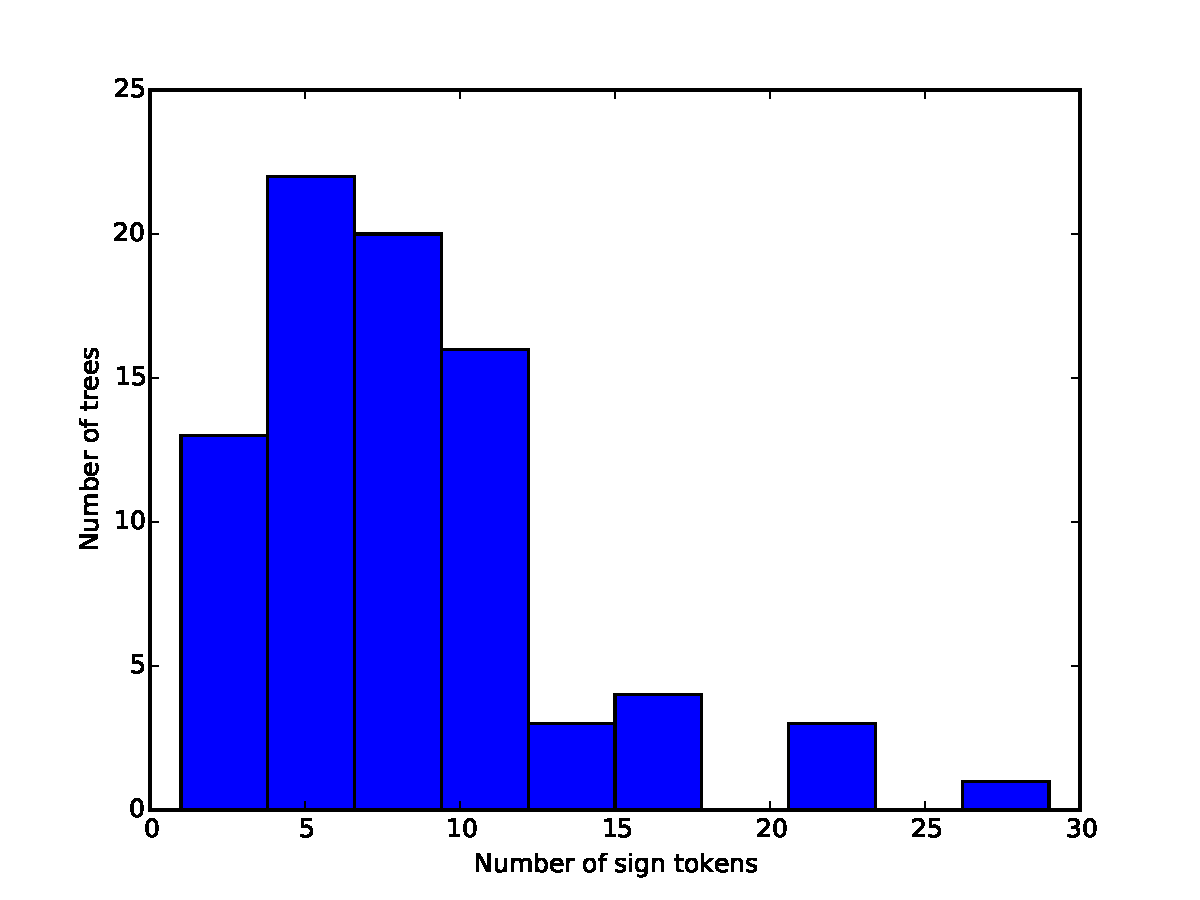
\includegraphics[width=\linewidth]{treesizes.pdf}
    \caption{Distribution of tree sizes for the Swedish Sign
        Language Universal Dependencies treebank.}
	\label{fig:treesizes}
\end{figure}

The SSL treebank released in version 1.4 of the UD treebanks contains 82 trees
with a total of 672 sign tokens (mean 8.2, median 7).  The distribution of
tree sizes (in tokens) is shown in \Fref{fig:treesizes}, as described in
\Fref{sec:annotation} these were produced in a bottom-up fashion and reflect
our judgment of the largest sensible syntactic segmentation of the material.
As could be expected from a corpus of spontaneous conversation, there is a
large number of small trees. For comparison, the only spoken language
(Slovenian) treebank has mean 9.1 and median 6, while the written Swedish
treebank %(a language which SSL has been in extensive contact with)
has mean 14.3 and median 13 sentence length, not counting punctuation.

\section{Dependency parsing}

Given that this is the first sign language UD treebank, we decided to perform
some dependency parsing experiments to establish baseline results.
We use the parser of \newcite{Straka2015parsito}, part of the UDpipe
toolkit \cite{Straka2016udpipe}, for our experiments. The training (334
tokens), development (48 tokens) and test (290 tokens) split from
UD treebanks 1.4 was used.
A hundred iterations of random hyperparameter search was performed for each of
their parser models (projective, partially non-projective and fully
non-projective), and the model with highest development set accuracy was
chosen.
Unsurprisingly given the small amount of training data, we found the most
constrained projective model performed best, in spite of the data containing
non-projective trees (see \Fref{fig:ssl_dep}).
Development set attachment score was 60 and 56 (unlabeled and labeled,
respectively) while the corresponding test set scores were 36 and
28. The discrepancy can be partly attributed to the much shorter mean
sentence length of the development set: 6.0 vs 10.4 for the test set.
Such low scores are not yet useful for practical tasks, but we emphasize that
our primary goal in this work is to explore the possibility of UD annotation
for a sign language. Our annotation project is ongoing, and we intend to
further expand the SSL part in future UD treebanks releases.

\section{Conclusions and future work}

In releasing the Universal Dependencies treebank of Swedish Sign Language
(SSL), the first such resource for a signed language,
we hope to enable new computational research into sign language syntax.
We have shown that even though some theoretical and practical issues exist
when applying UD principles to a sign language, it is possible to come up with
a reasonable annotation scheme. In the long run, we hope this will
stimulate the development of Natural
Language Processing (NLP) tools capable of processing sign languages.
Finally, because we have both parallel data in Swedish and language-independent
syntactic annotations, we also believe this resource could prove particularly
useful in cross-lingual NLP.


\section*{Acknowledgments}

Part of this work has been supported by an infrastructure grant from the
Swedish Research Council (SWE-CLARIN, project 821-2013-2003).


\bibliographystyle{acl}
\bibliography{nodalida2017ud}

\end{document}
